\documentclass[fleqn,a4paper,12pt]{article}

%used Packages
\usepackage{standalone}		% Zum Einlesen aus anderen .tex-Files
\usepackage{geometry}		% Zur Bearbeitung des Layouts (Ränder,...)
\usepackage[german]{babel}
\usepackage[utf8]{inputenc}
\usepackage{amsmath}		% Mathematische Symbole
\usepackage{amssymb}     	% Nochmehr mathematische Symbole
\usepackage{dsfont}      	% Schriftsatz fuer Zahlenmengensymbole
%\usepackage{verbatim}   	% erweiterte Verbatim-Umgebung
\usepackage{alltt}       	% Quasi-Verbatim-Umgebung
\usepackage{fancyhdr}    	% Eigene Kopfzeilen
\usepackage{graphicx}    	% Zum Einbinden von Grafiken
							% Einbinden einer eps-Grafik geht so: includegraphics{path}
\usepackage{wrapfig}
\usepackage{lscape}
\usepackage{rotating}
\usepackage{epstopdf}

% Skalierung der Grafiken
\setlength{\unitlength}{1cm}

\frenchspacing               % Kein Extrafreiraum nach Satzzeichen
\setlength{\parindent}{0pt}  % Neue Absaetze nicht einruecken
%\sloppy                     % Schlampige Absatzformatierung
\fussy                       % Penible Absatzformatierung
\linespread{1.5}             % Zeilenabstand


% Seitenraender
\geometry{left=30mm, right=40mm, bottom=30mm}
				% Doc-class, Packageimports, fancy stuff
%%Seitenränder formatieren
\addtolength{\voffset}{-2cm}
\addtolength{\textheight}{0cm}
\addtolength{\hoffset}{0cm}
\addtolength{\textwidth}{2cm}
\addtolength{\headheight}{2cm} % fuer jeden Strichkode einen Zentimeter

% Font fuer Code 39
\font\xlix=wlc39 scaled 1200
\newcommand\barcode[1]{{\xlix@#1@}}

% Name, Matrikelnummer, Barcode
\newcommand\student[2]{
	\mbox{\scriptsize
		\begin{tabular}{@{}l@{}r@{}}
			\multicolumn{2}{@{}r@{}}{\barcode{#2}}\\
			#1&#2\\
		\end{tabular}}}

% Kopfzeile
\pagestyle{fancy}            % Eigene Kopfzeilen verwenden
\lhead{
	\small
	\textsc{Grundlagen der Signalverarbeitung \\
		WS 2017/2018 \\
		\"Ubung (\today)}
	\vfill}
\rhead{
	\begin{tabular}[b]{@{}rr@{}}
		\student{Philipp Badenhoop}{572693} &
		\student{Steven Lange}{568733} \\
		\student{Pascal Jochmann}{575056} &
		\student{Kevin Trogant}{572451}
\end{tabular}}			% Definition der Kopfzeile
%andere Definitionen
\providecommand{\R}{{\mathbb R}}
\providecommand{\N}{{\mathbb N}}
\providecommand{\Z}{{\mathbb Z}}
\providecommand{\Q}{{\mathbb Q}}
\providecommand{\C}{{\mathbb C}}
\providecommand{\F}{\mathcal{F}}
\providecommand{\less}{\setminus}
\providecommand{\inv}{{}^{-1}}
\providecommand{\Land}{\bigwedge}
\providecommand{\Lor}{\bigvee}			% Liste der zusätzlichen Commands und redefines

\begin{document}
	\section*{Aufgabe 24}
		\begin{itemize}
			\item[(a)] $T_A = 0.004s$\\
				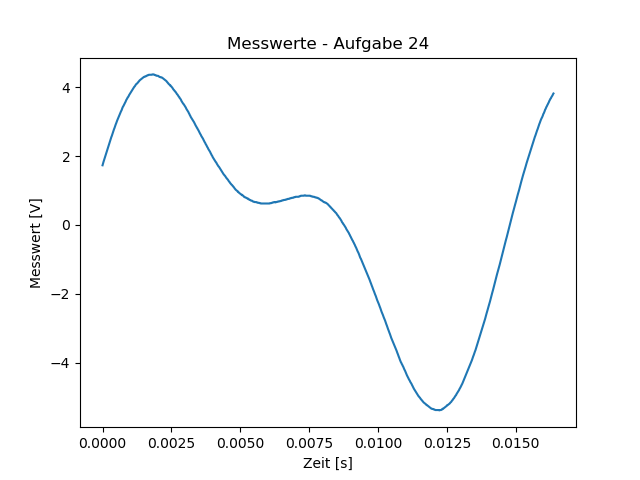
\includegraphics[scale = 0.7]{A24_messPlot.png}
			\item[(b)] $T_0 \approx 3.842s $\\
			$f_0 = \frac{1}{T_0} = 0.26Hz$\\
			$N = \left\lfloor \frac{3.842s}{0.004s} \right\rfloor = 960$\\
			$\omega_0 = \frac{2\pi}{N} \approx 0.0065\frac{rad}{s}$
			\item[(c)] Eine Periode mit $N$ Messwerte:\\
				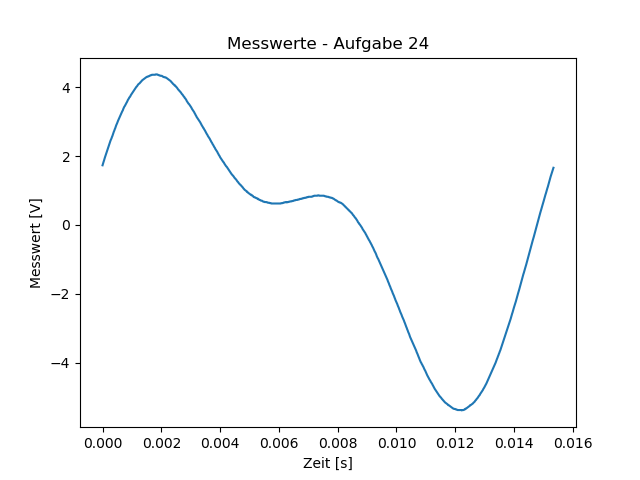
\includegraphics[scale = 0.7]{A24_messPlot_periode.png}
			\item[(d)] Für $k\in\{ 0, \pm 1, \pm 2, \dots \pm 15 \}$ gilt:
				$c_k = \frac{1}{960}\sum_{n=0}^{959} f_n\cdot e^{-j2\pi\frac{kn}{960}}$\\
			\begin{tabular}{c r r}
				k	&	$c_k$				&	$c_{-k}$\\
				0	&	-0.071				&	-0.071\\
				1	&	 0.226+1.809j		&	0.226-1.809j\\
				2	&	 0.667+0.772j		&	0.667-0.772j\\
				3	&	 0.000+0.003j		&	0.000-0.003j\\
				4	&	 0.000+0.001j		&	0.000-0.001j\\
				5	&	 0.000+0.001j		&	0.000-0.001j\\
				6	&	 0.001+0.001j		&	0.001-0.001j\\
				7	&	 0.001+0.000j		&	0.001+0.000j\\
				8	&	 0.001+0.000j		&	0.001+0.000j\\
				9	&	 0.001+0.001j		&	0.001-0.001j\\
				10	&	 0.000+0.000j		&	0.000+0.000j\\
				11	&	 0.000+0.001j		&	0.000-0.001j\\
				12	&	 0.000+0.001j		&	0.000-0.001j\\
				13	&	 0.000+0.001j		&	0.000-0.001j\\
				14	&	 0.000+0.000j		&	0.000+0.000j\\
				15	&	 0.000+0.001j		&	0.000-0.001j
			\end{tabular}
		\item[(d)] Das Linienspektrum sieht dann wie folgt aus:\\
			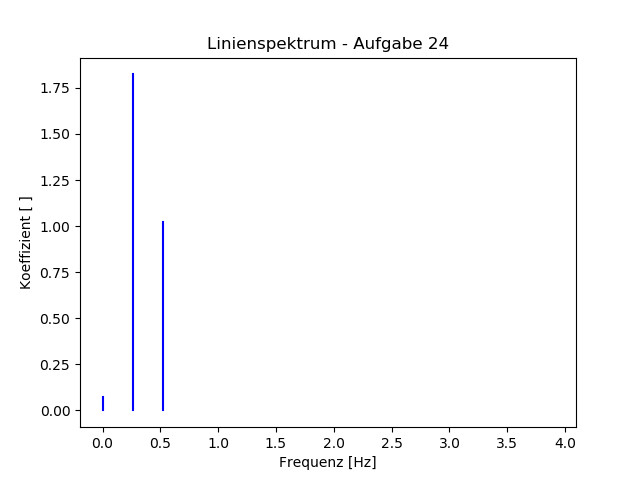
\includegraphics[scale = 0.7]{A24_Linienspektrum.png}
		\item[(e)] Das Signal ist zwar das Beispiel-Signal aus der Vorlesung und der Übung, aber welches dies genau ist, ist uns unbekannt.	
	\end{itemize}
\end{document}